% This LaTeX was auto-generated from MATLAB code.
% To make changes, update the MATLAB code and export to LaTeX again.

\documentclass{article}

\usepackage[utf8]{inputenc}
\usepackage[T1]{fontenc}
\usepackage{lmodern}
\usepackage{graphicx}
\usepackage{color}
\usepackage{listings}
\usepackage{hyperref}
\usepackage{amsmath}
\usepackage{amsfonts}
\usepackage{epstopdf}
\usepackage{matlab}

\sloppy
\epstopdfsetup{outdir=./}
\graphicspath{ {./main_images/} }

\begin{document}

\matlabtitle{Homework Assignment \# 7}

\begin{par}
\begin{flushleft}
\textbf{Carlos Rangel}
\end{flushleft}
\end{par}

\begin{matlabcode}
% This file implements the Algorithm described on page 3

% Initial Guess for p and V0
params;
pnew=(1/2)*(NU+repmat(c,1,L));
Vnew=(pnew-repmat(c,1,L))./(1-BETA);

% Stopping Criteria
eps=1e-3;

% Counter for iterations
iter=0;

% To enter first iteration
diff=10000;

% dampening parameter
lambda=1;
\end{matlabcode}
\begin{matlaboutput}
lambda = 1
\end{matlaboutput}


\begin{par}
\begin{flushleft}
Enter the loop and perform the necessary iterations until convergence
\end{flushleft}
\end{par}

\begin{matlabcode}
% Options
options=optimoptions('fsolve', 'Display', 'none');
while diff>eps
 Vold=Vnew;
 pold=pnew;
 % Obtain updated value for the prices
 
 % Set strategy for player 2
 p2=pold';
 
 % Define first order conditions given this strategy for player 2
 fun=@(p1) focs(p1, p2, Vold);
 
 % Update prices
 pnew=fsolve(fun, pold, options);
 
 % Update the Value of V
 Vnew=NextV(pnew,p2, Vold);
 
 % Compute maximum differences between Values and Policies
 diff=max( max(max( abs(Vnew-Vold)./(1+abs(Vnew)))), max(max(abs(pnew-pold)./(1+abs(pnew)))));
 
 % Dampening
 Vnew=lambda*Vnew+(1-lambda)*Vold;
 pnew=lambda*pnew+(1-lambda)*pold;
 
 % Increase Number of iterations
 iter=iter+1;
 
end
iter
\end{matlabcode}
\begin{matlaboutput}
iter = 122
\end{matlaboutput}
\begin{matlabcode}
diff
\end{matlabcode}
\begin{matlaboutput}
diff = 9.2252e-04
\end{matlaboutput}


\begin{par}
\begin{flushleft}
Plot the Value Function and Policy Function
\end{flushleft}
\end{par}

\begin{matlabcode}
% Value Function Plot
surf(omegas,omegas, Vnew)
\end{matlabcode}
\begin{center}
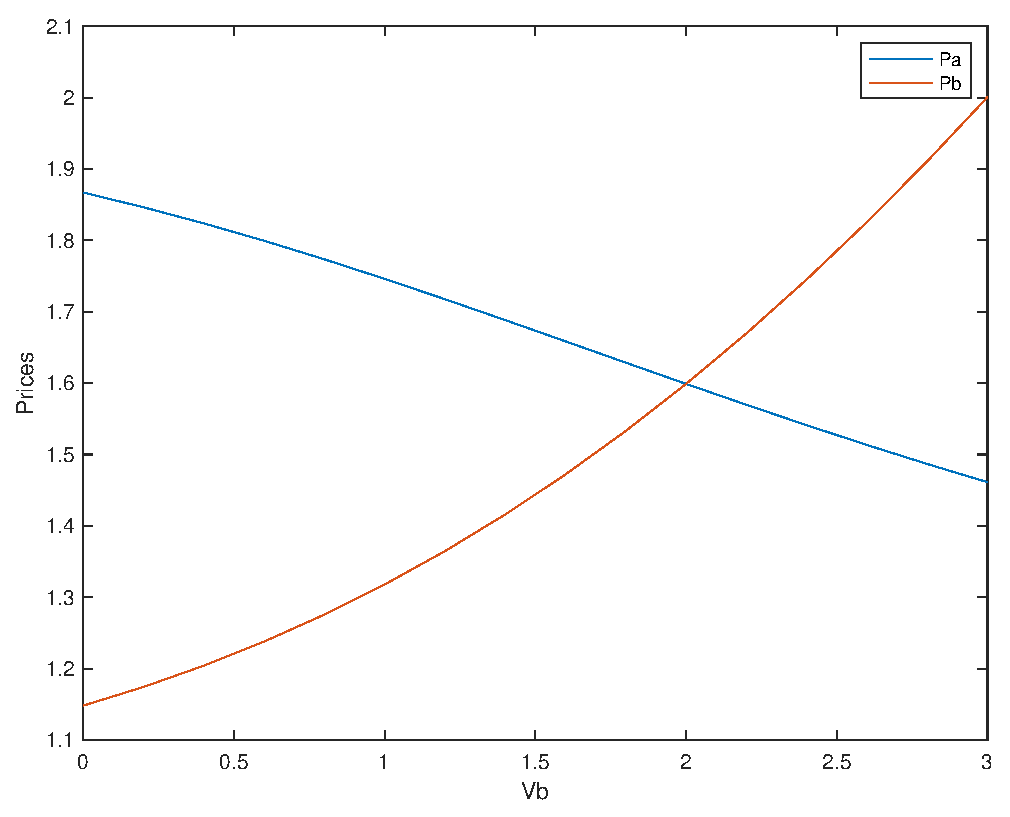
\includegraphics[width=\maxwidth{56.196688409433015em}]{figure_0}
\end{center}
\begin{matlabcode}

% Policy function plot
surf(omegas, omegas, pnew)
\end{matlabcode}
\begin{center}
\includegraphics[width=\maxwidth{56.196688409433015em}]{figure_1}
\end{center}


\matlabheading{Q2. Starting from state (1,1), plot the distribution of states a three dimensional plot) after 10, 20, and 30 periods.}

\begin{matlabcode}
% Calculate D1
D1=getD(pnew, pnew');

% Calculate D2
D2=getD(pnew', pnew);

% Calculate D0
D0=1./(1+exp(NU-pnew)+exp(NU-pnew'));

% Convert the D's into ((L*L) x 1) vectors
D1_vector=reshape(D1',L*L,1);
D2_vector=reshape(D2',L*L,1);
D0_vector=reshape(D0',L*L,1);

% Calculate Transition Probabilities for (q1,q2)=(1,0)
P_1_0=kron(PI(:,:,2), PI(:,:,1));

% Calculate Transition Probabilities for (q1,q2)=(0,1)
P_0_1=kron(PI(:,:,1), PI(:,:,2));

% Calculate Transition Probabilities for (q1, q2)=(0,0)
P_0_0=kron(PI(:,:,1), PI(:,:,1));

% Calculate final transition Probability P
P=D1_vector.*P_1_0 + D2_vector.*P_0_1 + D0_vector.*P_0_0;

% Create initial distribution
q=zeros(1, L*L);
q(1,1)=2;

% Distribution of states after 10 periods
q10=q*(P^10);

% As a matrix
q10_matrix=reshape(q10,L,L)';

% Distribution of states after 20 periods
q20=q*(P^20);

% As a matrix
q20_matrix=reshape(q20,L,L)';

% Distribution of states after 30 periods
q30=q*(P^30);

% As a matrix
q30_matrix=reshape(q30,L,L)';

% Plot these distributions

% For q10
surf(omegas, omegas, q10_matrix)
\end{matlabcode}
\begin{center}
\includegraphics[width=\maxwidth{56.196688409433015em}]{figure_2}
\end{center}
\begin{matlabcode}

% For q20
surf(omegas, omegas, q20_matrix)
\end{matlabcode}
\begin{center}
\includegraphics[width=\maxwidth{56.196688409433015em}]{figure_3}
\end{center}
\begin{matlabcode}

% For q30
surf(omegas, omegas, q30_matrix)
\end{matlabcode}
\begin{center}
\includegraphics[width=\maxwidth{56.196688409433015em}]{figure_4}
\end{center}


\matlabheading{Compute and plot the stationary distribution of states}

\begin{matlabcode}
% Criteria for finding a distribution that converges to a stationary one
eps_criteria=1e-5;

% Old distribution
q_old=q;

% New Distribution
q_new=q*(P^300);

% Difference between old and new distribution
diff_dist=max(abs(q_new-q_old));

while diff_dist>eps
    q_old=q_new;
    q_new=q_old*P;
    diff_dist=max(abs(q_new-q_old))
end
\end{matlabcode}
\begin{matlaboutput}
diff_dist = 1.4345e-05
\end{matlaboutput}
\begin{matlabcode}
q_stat=q_new;

% As a matrix
q_stat_matrix=reshape(q_new,L,L)';

% Plot
surf(omegas, omegas, q_stat_matrix);
\end{matlabcode}
\begin{center}
\includegraphics[width=\maxwidth{56.196688409433015em}]{figure_5}
\end{center}

\end{document}
